\documentclass[../../../../../../../dd.tex]{subfiles}

\begin{document}

	\subsubsection{Zones Manager}
		This component contains all the sub-components needed to manage zones and taxi queues.
		It provide some functions to get avaialables Taxi Drivers and to notify that a Taxi Driver has been chosen for a ride.
		\begin{itemize}
			\item \textbf{Zone Calculator:} The only function of this sub-component is to return the zone associated to a certain position.

			\item \textbf{Queues Manager:} This sub-component is in charge to keep the queues updated and to provide functions to select Taxi Driver from them.

			\item \textbf{GPS Updater:} This sub-component is in charge to receive GPS updates from IO Manager and to ask to the Database Manager to update them.
		\end{itemize}

		\begin{figure}[H]
				\centering
				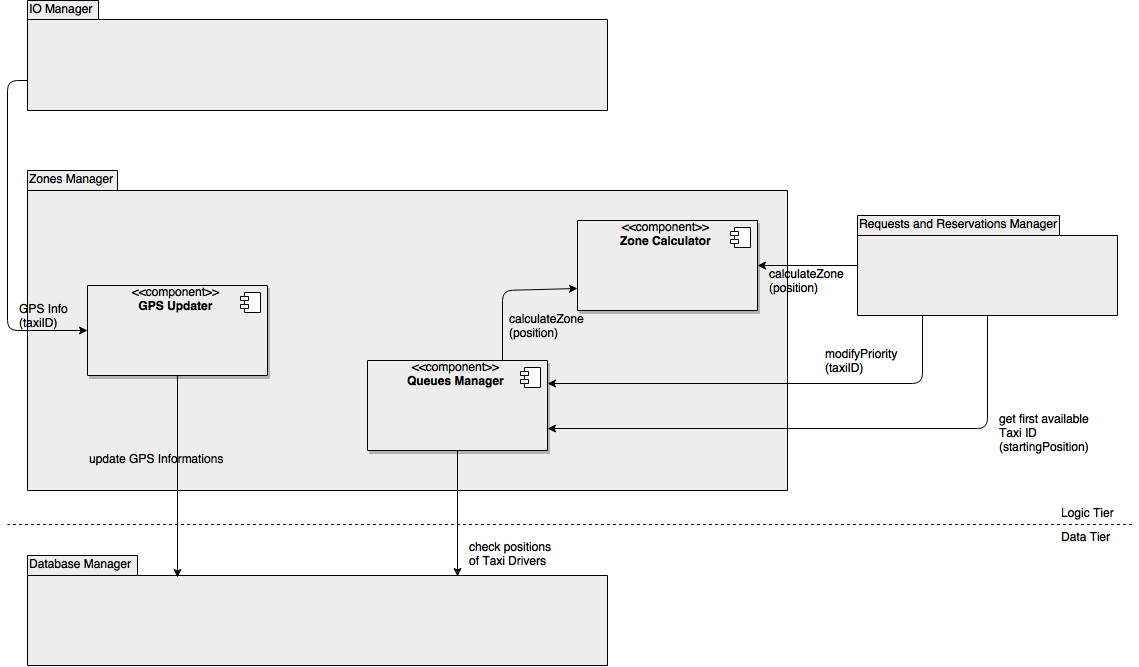
\includegraphics[width=\textwidth, scale=0.5]{../images/ZonesManager.png}
			\caption{Zones Manager Structure}\label{fig:ZonesManager}
		\end{figure}
		
\end{document}